\documentclass{article}

\usepackage{tikz} 
\usetikzlibrary{automata, positioning, arrows} 

\usepackage{amsthm}
\usepackage{amsfonts}
\usepackage{amsmath}
\usepackage{amssymb}
\usepackage{fullpage}
\usepackage{color}
\usepackage{parskip}
\usepackage{hyperref}
\usepackage{graphicx}
\usepackage{listings}
\usepackage{tikz-cd}
\usepackage{textalpha}
  \hypersetup{
    colorlinks = true,
    urlcolor = blue,       % color of external links using \href
    linkcolor= blue,       % color of internal links 
    citecolor= blue,       % color of links to bibliography
    filecolor= blue,        % color of file links
    }
    
\usepackage{listings}

\lstset{escapeinside={(*@}{@*)}}

\definecolor{dkgreen}{rgb}{0,0.6,0}
\definecolor{gray}{rgb}{0.5,0.5,0.5}
\definecolor{mauve}{rgb}{0.58,0,0.82}

\lstset{frame=tb,
  language=haskell,
  aboveskip=3mm,
  belowskip=3mm,
  showstringspaces=false,
  columns=flexible,
  basicstyle={\small\ttfamily},
  numbers=none,
  numberstyle=\tiny\color{gray},
  keywordstyle=\color{blue},
  commentstyle=\color{dkgreen},
  stringstyle=\color{mauve},
  breaklines=true,
  breakatwhitespace=true,
  tabsize=3
}

\newtheoremstyle{theorem}
  {\topsep}   % ABOVESPACE
  {\topsep}   % BELOWSPACE
  {\itshape\/}  % BODYFONT
  {0pt}       % INDENT (empty value is the same as 0pt)
  {\bfseries} % HEADFONT
  {.}         % HEADPUNCT
  {5pt plus 1pt minus 1pt} % HEADSPACE
  {}          % CUSTOM-HEAD-SPEC
\theoremstyle{theorem} 
   \newtheorem{theorem}{Theorem}[section]
   \newtheorem{corollary}[theorem]{Corollary}
   \newtheorem{lemma}[theorem]{Lemma}
   \newtheorem{proposition}[theorem]{Proposition}
\theoremstyle{definition}
   \newtheorem{definition}[theorem]{Definition}
   \newtheorem{example}[theorem]{Example}
\theoremstyle{remark}    
  \newtheorem{remark}[theorem]{Remark}

\title{CPSC-354 Report}
\author{Maxwell Rovenger  \\ Chapman University}

\date{\today} 

\begin{document}

\maketitle

\begin{abstract}
% (Delete and Replace:) You can safely delete and replace the explanations in this file as they will remain available on the course website. For example, you should replace this abstract with your own. The abstract should be a short summary of the report. It should be written in a way that makes it possible to understand the purpose of the report without reading it.  
\end{abstract}

\setcounter{tocdepth}{3}
\tableofcontents

\section{Introduction}\label{intro}

(Delete and Replace): This report will document your learning throughout the course. It will be a collection of your notes, homework solutions, and critical reflections on the content of the course. Something in between a semester-long take home exam and your own lecture notes.\footnote{One purpose of giving the report the form of lecture notes is that self-explanation is a technique proven to help with learning, see Chapter 6 of Craig Barton, How I Wish I'd Taught Maths, and references therein. In fact, the report can lead you from self-explanation (which is what you do for the weekly deadline) to explaining to others (which is what you do for the final submission). Another purpose is to help those of you who want to go on to graduate school to develop some basic writing skills. A report that you could proudly add to your application to graduate school (or a job application in industry) would give you full points.}

To modify this template you need to modify the source \texttt{report.tex} which is available in the course repo. For guidance on how to do this read both the source and the pdf of \texttt{latex-example.tex} which is also available in the repo. Also check out the usual resources (Google, Stackoverflow, LLM, etc). It was never as easy as now to learn a new programming lanugage (which, btw, \LaTeX{} is).

For writing \LaTeX{} with VSCode use the \href{https://marketplace.visualstudio.com/items?itemName=James-Yu.latex-workshop}{LaTeX Workshop} extension. 

There will be deadlines during the semester, graded mostly for completeness. That means that you will get the points if you submit in time and are on the right track, independently of whether the solutions are technically correct. You will have the opportunity to revise your work for the final submission of the full report.

The full report is due at the end of the finals week. It will be graded according to the following guidelines.

\section{Week by Week}\label{homework}

\subsection{Week 1}

\subsubsection*{Notes}

Lectures introduced Lean, a programming language to help prove discrete mathematics proofs. Through using the Natural Numbers Game, we saw how Lean operates and how it works it can, with functions acting as steps, prove theorems similar to how we did in discrete math with pen and paper and induction.

\subsubsection*{Homework}

Solved problems in Natural Numbers Game using Lean to help recap teachings from Discrete Mathematics. Specifically dealing with successors and predecessors and how they can be used to change certain sides to equal the other.

Level 5/8:
\begin{lstlisting}
a + (b + 0) + (c + 0) = a + b + c
rw [add_zero]
a + b + (c + 0) = a + b + c
rw [add_zero]
a + b + c = a + b + c
rfl
\end{lstlisting}

Level 6/8:
\begin{lstlisting}
a + (b + 0) + (c + 0) = a + b + c
rw[add_zero c]
a + (b + 0) + c = a + b + c
rw[add_zero b]
a + b + c = a + b + c
rfl
\end{lstlisting}

Level 7/8:
\begin{lstlisting}
succ n = n + 1
rw[one_eq_succ_zero]
succ n = n + succ 0
rw[add_succ]
succ n = succ (n + 0)
rw[add_zero]
succ n = succ n
rfl
\end{lstlisting}

Level 8/8:
\begin{lstlisting}
2 + 2 = 4
rw[four_eq_succ_three]
2 + 2 = succ 3
rw[three_eq_succ_two]
2 + 2 = succ (succ 2)
rw[two_eq_succ_one]
succ 1 + succ 1 = succ (succ (succ 1))
rw[add_succ]
succ (succ 1 + 1) = succ (succ (succ 1))
rw[succ_eq_add_one]
succ 1 + 1 + 1 = succ (succ (succ 1))
rw[succ_eq_add_one]
1 + 1 + 1 + 1 = succ (succ (1 + 1))
rw[succ_eq_add_one]
1 + 1 + 1 + 1 = succ (1 + 1) + 1
rw[succ_eq_add_one]
1 + 1 + 1 + 1 = 1 + 1 + 1 + 1
rfl
\end{lstlisting}

For level 5/8 specifically, we can see that the Lean proof, \texttt{rw[add\_zero]}, corresponds to Proof Algorithm 1: Addition, in that any variable added to zero will ultimately equal just the variable. For example: $a + 0 = a$.

From this homework, I learned how to use the Lean proof and saw how each function operated exactly like algorithms and proofs I had used in Discrete Mathematics.

%In case you want to draw automata in Latex, you can use the tikz %package. Here is an example of a simple automaton:
%
%\begin{tikzpicture}[shorten >=1pt,node distance=2cm,on grid,auto] 
%  \node[state] (q_1)   {$q_1$}; 
%  \node[state] (q_2) [above right=of q_1] {$q_2$}; 
%  \node[state] (q_3) [below right=of q_2] {$q_3$}; 
%   \path[->] 
%   (q_1) edge  node {0} (q_2)
%         edge  node [swap] {1} (q_3)
%   (q_2) edge  node  {1} (q_3)
%         edge [loop above] node {0} ()
%   (q_3) edge [loop below] node {0,1} ();
%\end{tikzpicture}
%
%By the way, GPT-4 is quite good at outputting tikz code.

\subsubsection*{Comments and Questions}

Although this week generally served as just an introduction to the curriculum and a recap of discrete mathematics, I am curious as to whether or not there was a better example to be shown of how exactly a computer uses discrete mathematics. At this point, I am knowledgeable of how discrete mathematics operates and how computers can use operators to conduct mathematical operations, but I have yet to see a direct example of a computer "thinking" through a math calculation.

If the way computers have been taught mathematics is based purely on successors and predecessors, does that make other operations like multiplication, division, and exponents far more taxing on a CPU since they have to calculate an incredible amount of successors, or do the operators used to cause multiplication and exponentiation ignore that by just creating duplicates and adding them together?

%I expect you to read the lecture notes. 

\subsection{Week 2}

\subsubsection*{Notes}

Recursion, in coding, allows for more simplistic code that is easier to read, scale, and apply. 

Regarding the allowing of typos in coding, code should be non-ambigious because coding should be universal and should work the same within the same virtual machine regardless of how you access it. We see examples of this in GitHub's copilot since it only makes suggestions that are non-ambigious and can work on any machine, as long as they have the correct virtual machine.

Lean contains tactics, Ex: rw, and theorems, Ex: one\_eq\_succ\_zero. Tactics are commands while theorems are logical propositions.

\subsubsection*{Homework}
Level 1/5:
\begin{lstlisting}
0 + n = n
induction n with d hd
0 + 0 = 0
rw[add_zero]
0 = 0
rfl
0 + succ d = succ d
rw[add_succ]
succ (0 + d) = succ d
rw[hd]
succ d = succ d
rfl
\end{lstlisting}

Level 2/5:
\begin{lstlisting}
succ a + b = succ (a + b)
induction b with b
succ a + 0 = succ (a + 0)
rw[add_zero]
succ a = succ (a + 0)
rw[add_zero]
succ a = succ a
rfl
succ a + succ b = succ (a + succ b)
rw[add_succ]
succ (succ a + b) = succ (a + succ b)
rw[n_ih]
succ (succ (a + b)) = succ (a + succ b)
rw[add_succ]
succ (succ (a + b)) = succ (succ (a + b))
rfl
\end{lstlisting}

Level 3/5:
\begin{lstlisting}
a + b = b + a
induction b with b hb
a + 0 = 0 + a
rw [add_zero]
a = 0 + a
rw [zero_add]
a = a
rfl
a + succ b = succ b + a
rw [add_succ]
succ (a + b) = succ b + a
rw [hb]
succ (b + a) = succ b + a
rw [succ_add]
succ (b + a) = succ (b + a)
rfl
\end{lstlisting}

Level 4/5:
\begin{lstlisting}
a + b + c = a + (b + c)
induction c with c hc
a + b + 0 = a + (b + 0)
rw [add_zero]
a + b = a + (b + 0)
rw [add_zero]
a + b = a + b
rfl
a + b + succ c = a + (b + succ c)
rw [add_succ]
succ (a + b + c) = a + (b + succ c)
rw [add_succ]
succ (a + b + c) = a + succ (b + c)
rw [add_succ]
succ (a + b + c) = succ (a + (b + c))
rw [hc]
succ (a + (b + c)) = succ (a + (b + c))
rfl
\end{lstlisting}

Level 5/5:
\begin{lstlisting}
a + b + c = a + c + b
induction c with c hc
a + b + 0 = a + 0 + b
rw [add_zero, add_zero]
a + b = a + b
rfl
a + b + succ c = a + succ c + b
rw [add_succ]
succ (a + b + c) = a + succ c + b
rw [add_succ]
succ (a + b + c) = succ (a + c) + b
rw [succ_add]
succ (a + b + c) = succ (a + c + b)
rw [hc]
succ (a + c + b) = succ (a + c + b)
rfl
\end{lstlisting}
\subsubsection*{Comments and Questions}

Personally, I felt that when it comes to AI autocorrecting code, instead of being lenient towards mistyped code, AI could just simply correct the typos. This would allow for a smoother coding process wihle also creating non-ambigious code.

After playing around with the Tower of Hanoi, it is apparent that recursion is invaluable in programming. We often see it as a way to neatly write code but it can also be massive time saver as apparent with the Tower of Hanoi where instead of having to, through trial and error finding out the solution, we can just use a recursive equation and plug in our values. My question then is, in what other fields can we apply recursion, as it is becoming more apparent to me that recursion can be a form of thinking rather than a field specific method?

\subsubsection*{Lean Proof}

\begin{align*}
  a + b + c = a + (b + c) \\
  a + b + 0 = a + (b + 0) == def of + \\
  a + b = a + (b + 0) == def of + \\
  a + b = a + b \\
\end{align*}

\subsection{Week 3}

\subsubsection*{Notes}

It is impossible for a computer to prove all mathematical proofs since there are statements in arithmetic that are unclear if they are true or not and thus cannot be proved. This is due to there being proofs in mathematics that are built based upon assumption and although there are no problems found so far, they cannot be proved through ordinary means like what the computer would opt to do.

\subsubsection*{Homework}

\href{https://github.com/mrovengerdev/LLM-literature-review/blob/main/README.md}{LLM Literature Review README}

\subsubsection*{Discord Posting}

For my literature review, I used ChatGPT4 to ask questions about recursion within computer systems. More specifically, if it decreases memory usage or provides any processing speed based benefits rather than just readability or integration based benefits. Through my conversation, I learned that due to creating more and more stack frames for each iteration, recursion can actually increase memory usage. However, there is an alternative, that being tail recursion. It was developed in 1970s however it either does not have support or only has limited support for popular languages like Python and JavaScript. Thus, it was concluded that recursive functions are actually less memory efficient than iterative solutions. This surprised me as through recursion, humans are able to abstract a lot of our thinking and are able to quickly find out what the next iterative output is. This contrasts computers which require more processing power to perform recursive methods. This creates an inverse relationship where the better the human understanding, the worse the computer understanding.

\subsection{Week 4}

\subsubsection*{Notes}

An abstract syntax tree is the result of parsing and helps display the order and relationship between operators in a mathematical problem. the abstract syntax tree is the most intermediate, as it is more drawn out than both concrete syntax and a concrete syntax tree.

We can define well formed expressions through formal grammar. Since formal grammar helps to create definitions for what becomes a well-formed expression.

\subsubsection*{Homework}

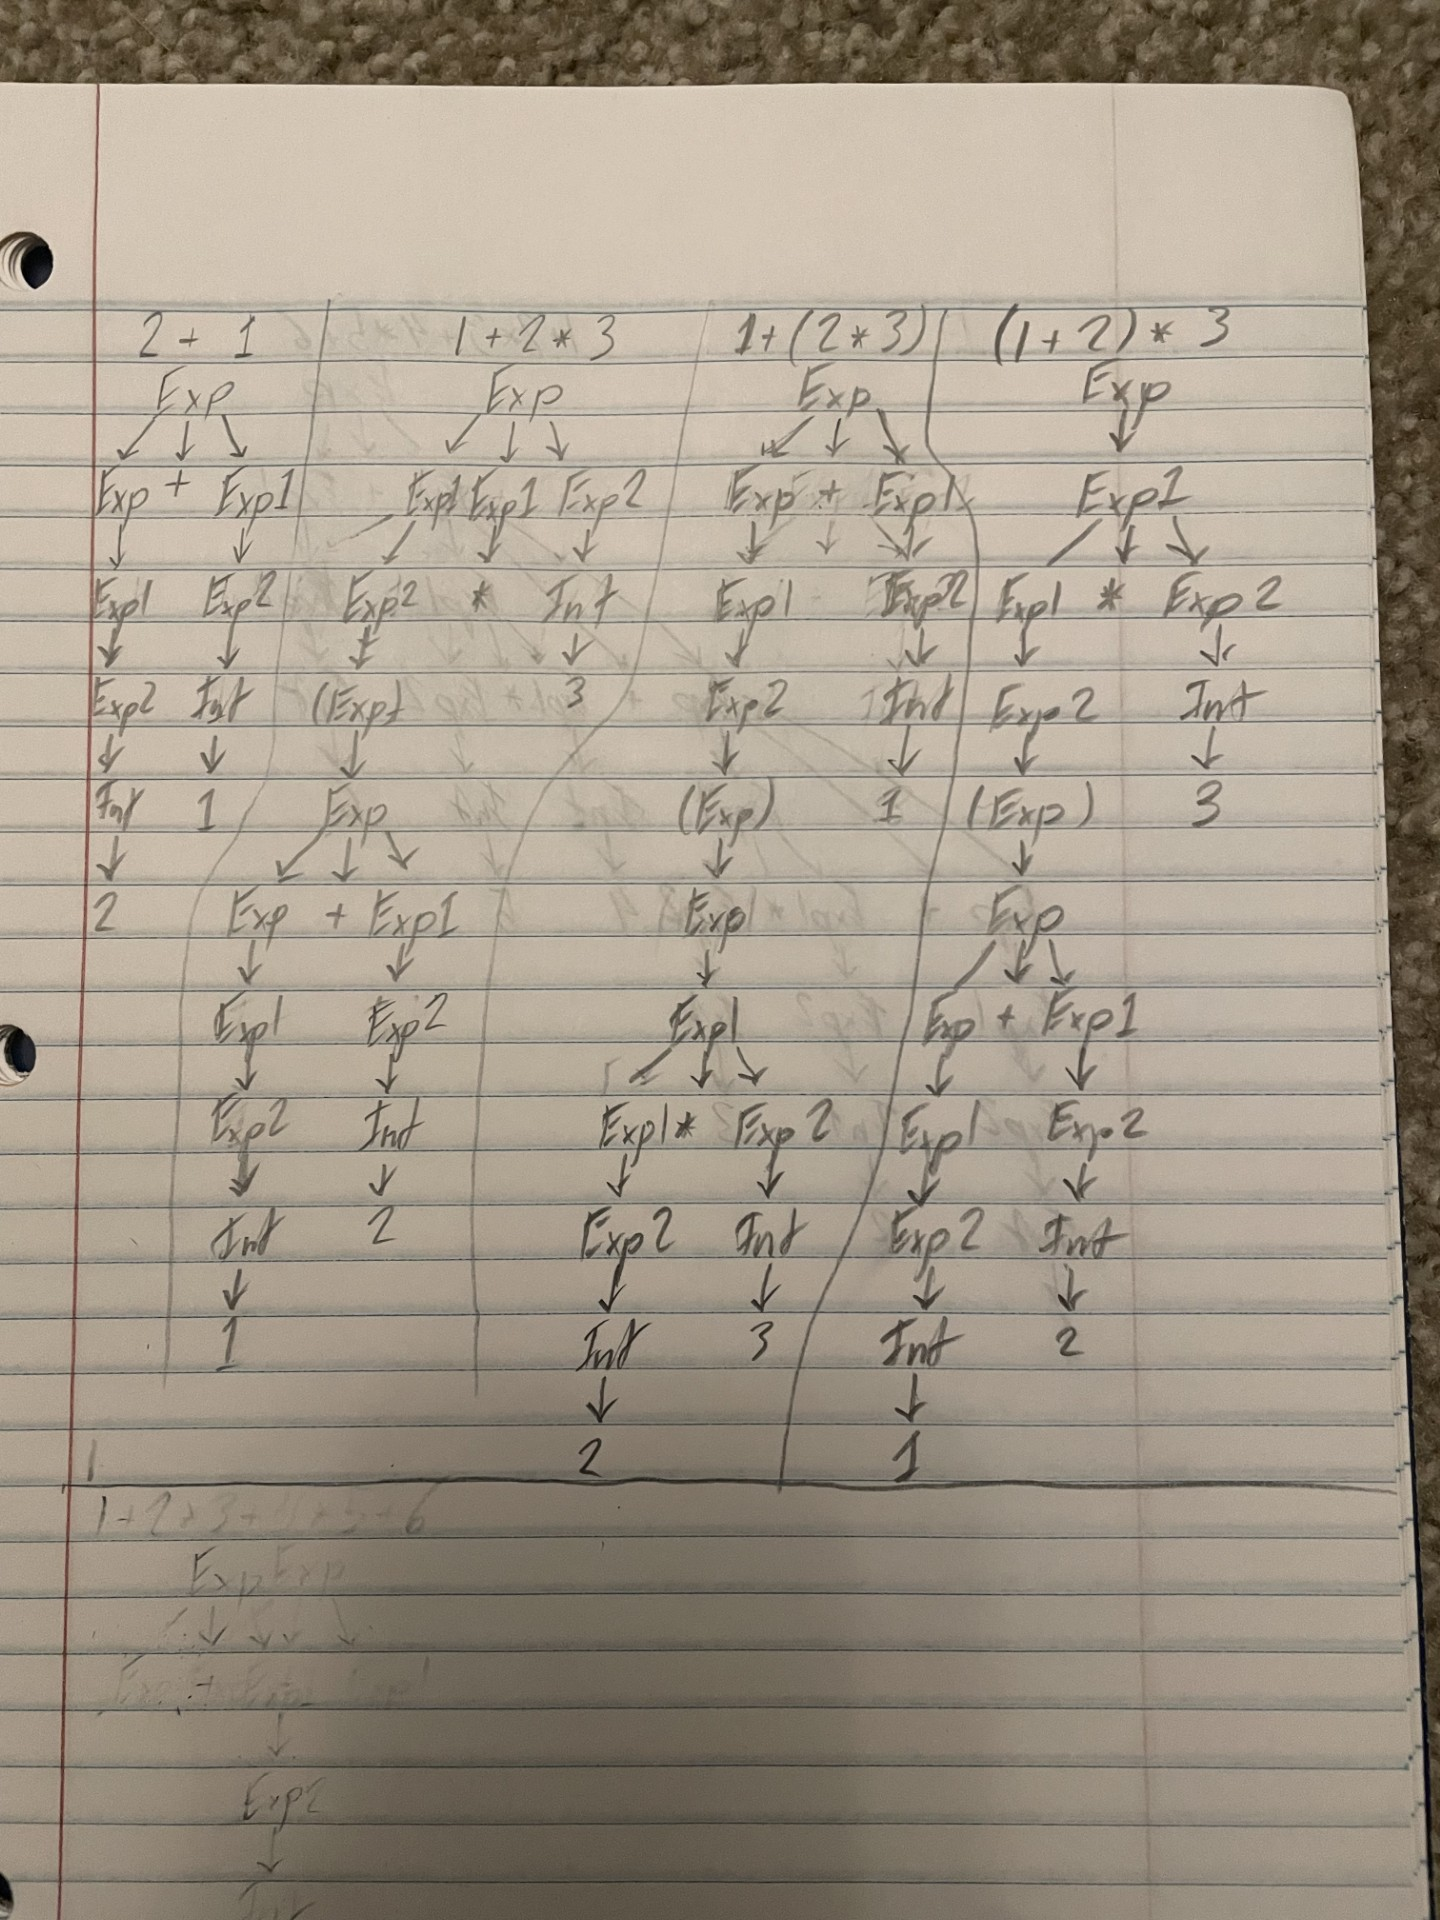
\includegraphics[width=0.45\textwidth]{HW4IMG1.jpg}
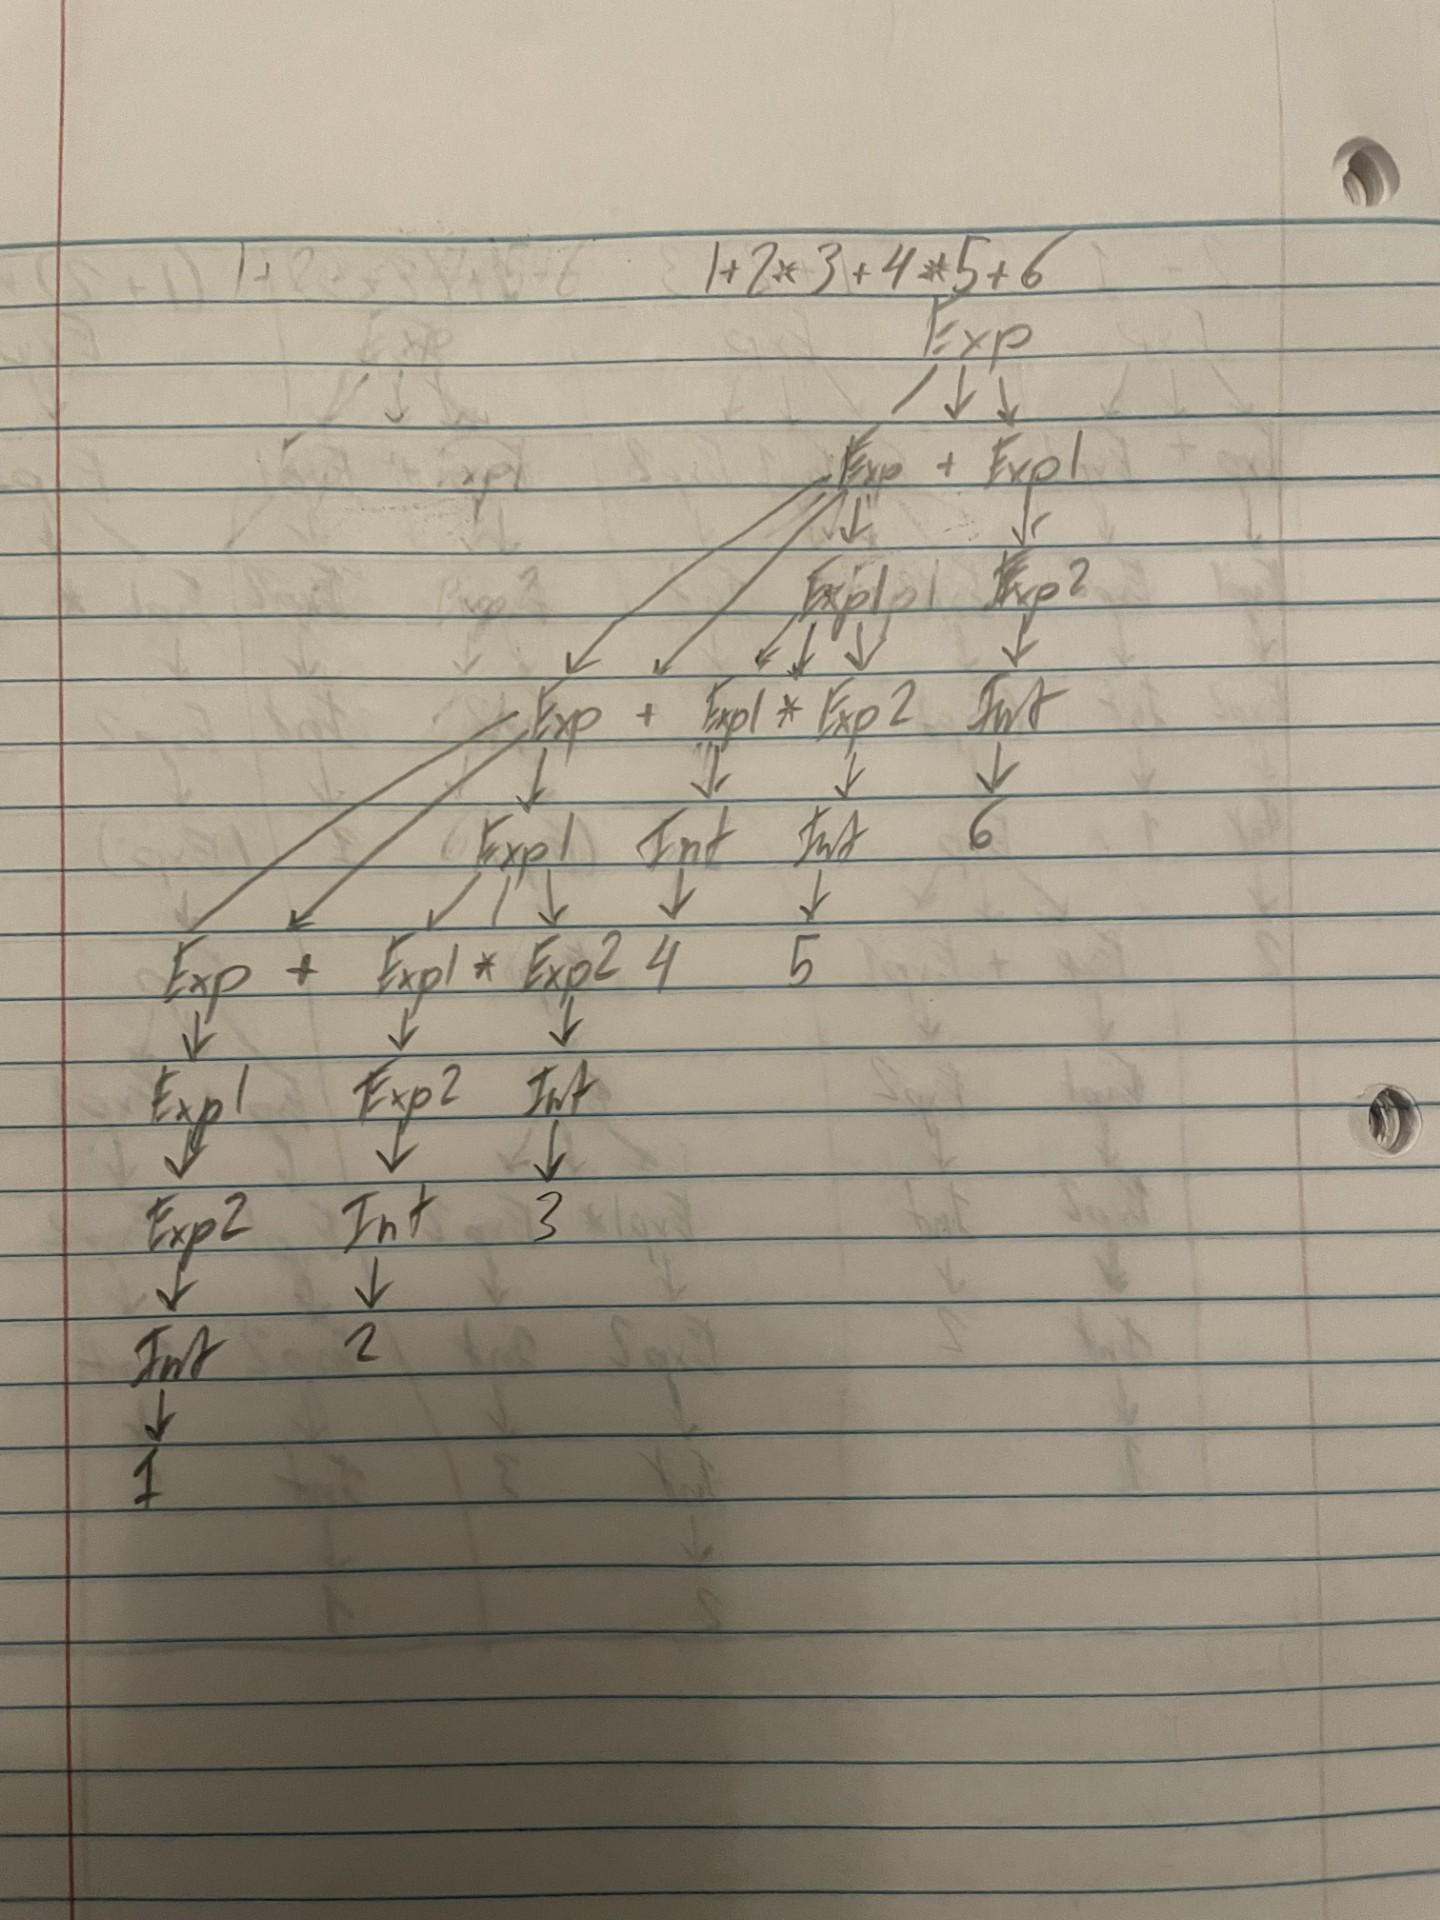
\includegraphics[width=0.45\textwidth]{HW4IMG2.jpg}

\subsubsection*{Questions and Comments}

If my understanding is correct, all formal languages are allowed to have their own alphabets and grammar that must be defined. However, we have found ourselves in a position where the majority of, if not all, programming langauges will use the same characters or symbols for operators and values. Thus, my question is if there is a protocol enforced that mandates the formal language used in a programming languages or has this all occurred just for ease of use?

\subsection{Week 5}

\subsubsection*{Notes}

In this week's lecture, we learned about the logic behind AND and how computer's process it. This shows that a proof in logic can be represented as a program in a programming language and vice versa.

Similarly, in the natural numbers game, we saw the application of these theorems which allowed us to prove theorems in Lean. So if a refresher is needed, going through the "A Lean Intro To Logic" is a good idea.

\subsubsection*{Homework}
Level 1/8:
\begin{lstlisting}
todo_list: P
exact todo_list
\end{lstlisting}

Level 2/8:
\begin{lstlisting}
(*@ $[ Goal: P \land S ]$ @*)
exact and_intro p s
\end{lstlisting}

Level 3/8:
\begin{lstlisting}
(*@ $[ Goal: (A \land I) \land O \land U ]$ @*)
exact and_intro (and_intro a i) (and_intro o u)
\end{lstlisting}

Level 4/8:
\begin{lstlisting}
Assumptions:
  (*@ $[ - vm: P \land S ]$ @*)
have p := vm.left
Assumptions: 
  (*@ $[ - vm: P \land S ]$ @*)
  (*@ $[ - p: P ]$ @*)
exact p
\end{lstlisting}

Level 5/8:
\begin{lstlisting}
Assumptions:
  (*@ $[ - h: P \land Q ]$ @*)
have q := and_right h
Assumptions:
  (*@ $[ - h: P \land Q ]$ @*)
  (*@ $[ - q: Q ]$ @*)
exact q
\end{lstlisting}

Level 6/8:
\begin{lstlisting}
Assumptions:
  (*@ $[ - h1: A \land I ]$ @*)
  (*@ $[ - h2: O \land U ]$ @*)
have A := and_left h1
Assumptions:
  (*@ $[ - h1: A \land I ]$ @*)
  (*@ $[ - h2: O \land U ]$ @*)
  (*@ $[ - A: A ]$ @*)
have U := and_right h2
Assumptions:
  (*@ $[ - h1: A \land I ]$ @*)
  (*@ $[ - h2: O \land U ]$ @*)
  (*@ $[ - A: A ]$ @*)
  (*@ $[ - U: U ]$ @*)
exact and_intro A U
\end{lstlisting}

Level 7/8:
\begin{lstlisting}
Assumptions:
  (*@ $[ - h: (L \land ((L \land C) \land L) \land L \land L \land L) \land (L \land L) \land L ]$ @*)
have h1 := and_left h
Assumptions:
  (*@ $[ - h: (L \land ((L \land C) \land L) \land L \land L \land L) \land (L \land L) \land L ]$ @*)
  (*@ $[ - h1: L \land ((L \land C) \land L) \land L \land L \land L ]$ @*)
have h2 := and_right h1
Assumptions:
  (*@ $[ - h: (L \land ((L \land C) \land L) \land L \land L \land L) \land (L \land L) \land L ]$ @*)
  (*@ $[ - h1: L \land ((L \land C) \land L) \land L \land L \land L ]$ @*)
  (*@ $[ - h2: ((L \land C) \land L) \land L \land L \land L ]$ @*)
have h3 := and_left h2
Assumptions:
  (*@ $[ - h: (L \land ((L \land C) \land L) \land L \land L \land L) \land (L \land L) \land L ]$ @*)
  (*@ $[ - h1: L \land ((L \land C) \land L) \land L \land L \land L ]$ @*)
  (*@ $[ - h2: ((L \land C) \land L) \land L \land L \land L ]$ @*)
  (*@ $[ - h3: (L \land C) \land L ]$ @*)
have h4 := and_left h3
Assumptions:
  (*@ $[ - h: (L \land ((L \land C) \land L) \land L \land L \land L) \land (L \land L) \land L ]$ @*)
  (*@ $[ - h1: L \land ((L \land C) \land L) \land L \land L \land L ]$ @*)
  (*@ $[ - h2: ((L \land C) \land L) \land L \land L \land L ]$ @*)
  (*@ $[ - h3: (L \land C) \land L ]$ @*)
  (*@ $[ - h4: L \land C ]$ @*)
have h5 := and_right h4
Assumptions:
  (*@ $[ - h: (L \land ((L \land C) \land L) \land L \land L \land L) \land (L \land L) \land L ]$ @*)
  (*@ $[ - h1: L \land ((L \land C) \land L) \land L \land L \land L ]$ @*)
  (*@ $[ - h2: ((L \land C) \land L) \land L \land L \land L ]$ @*)
  (*@ $[ - h3: (L \land C) \land L ]$ @*)
  (*@ $[ - h4: L \land C ]$ @*)
  (*@ $[ - h5: C ]$ @*)
exact h5
\end{lstlisting}

Level 8/8:
\begin{lstlisting}
Assumptions:
  (*@ $[ - h: ((P \land S) \land A) \land \neg I \land (C \land \neg O) \land \neg U ]$ @*) and_left (1)
have h1 := and_left h
Assumptions:
  (*@ $[ - h: ((P \land S) \land A) \land \neg I \land (C \land \neg O) \land \neg U ]$ @*)
  (*@ $[ - h1: (P \land S) \land A ]$ @*)
have h2 := and_left h1
Assumptions:
  (*@ $[ - h: ((P \land S) \land A) \land \neg I \land (C \land \neg O) \land \neg U ]$ @*)
  (*@ $[ - h1: (P \land S) \land A ]$ @*)
  (*@ $[ - h2: P \land S ]$ @*)
have h3 := and_right h1
Assumptions:
  (*@ $[ - h: ((P \land S) \land A) \land \neg I \land (C \land \neg O) \land \neg U ]$ @*)
  (*@ $[ - h1: (P \land S) \land A ]$ @*)
  (*@ $[ - h2: P \land S ]$ @*)
  (*@ $[ - h3: A ]$ @*)
have h4 := and_right h
Assumptions:
  (*@ $[ - h: ((P \land S) \land A) \land \neg I \land (C \land \neg O) \land \neg U ]$ @*)
  (*@ $[ - h1: (P \land S) \land A ]$ @*)
  (*@ $[ - h2: P \land S ]$ @*)
  (*@ $[ - h3: A ]$ @*)
  (*@ $[ - h4: \neg I \land (C \land \neg O) \land \neg U ]$ @*)
have h5 := and_right h4
Assumptions:
  (*@ $[ - h: ((P \land S) \land A) \land \neg I \land (C \land \neg O) \land \neg U ]$ @*)
  (*@ $[ - h1: (P \land S) \land A ]$ @*)
  (*@ $[ - h2: P \land S ]$ @*)
  (*@ $[ - h3: A ]$ @*)
  (*@ $[ - h4: \neg I \land (C \land \neg O) \land \neg U ]$ @*)
  (*@ $[ - h5: (C \land \neg O) \land \neg U ]$ @*)
have h6 := and_left h5
Assumptions:
  (*@ $[ - h: ((P \land S) \land A) \land \neg I \land (C \land \neg O) \land \neg U ]$ @*)
  (*@ $[ - h1: (P \land S) \land A ]$ @*)
  (*@ $[ - h2: P \land S ]$ @*)
  (*@ $[ - h3: A ]$ @*)
  (*@ $[ - h4: \neg I \land (C \land \neg O) \land \neg U ]$ @*)
  (*@ $[ - h5: (C \land \neg O) \land \neg U ]$ @*)
  (*@ $[ - h6: C \land \neg O ]$ @*)
have h7 := and_left h6
Assumptions:
  (*@ $[ - h: ((P \land S) \land A) \land \neg I \land (C \land \neg O) \land \neg U ]$ @*)
  (*@ $[ - h1: (P \land S) \land A ]$ @*)
  (*@ $[ - h2: P \land S ]$ @*)
  (*@ $[ - h3: A ]$ @*)
  (*@ $[ - h4: \neg I \land (C \land \neg O) \land \neg U ]$ @*)
  (*@ $[ - h5: (C \land \neg O) \land \neg U ]$ @*)
  (*@ $[ - h6: C \land \neg O ]$ @*)
  (*@ $[ - h7: C ]$ @*)
have h8 := and_left h2
Assumptions:
  (*@ $[ - h: ((P \land S) \land A) \land \neg I \land (C \land \neg O) \land \neg U ]$ @*)
  (*@ $[ - h1: (P \land S) \land A ]$ @*)
  (*@ $[ - h2: P \land S ]$ @*)
  (*@ $[ - h3: A ]$ @*)
  (*@ $[ - h4: \neg I \land (C \land \neg O) \land \neg U ]$ @*)
  (*@ $[ - h5: (C \land \neg O) \land \neg U ]$ @*)
  (*@ $[ - h6: C \land \neg O ]$ @*)
  (*@ $[ - h7: C ]$ @*)
  (*@ $[ - h8: P ]$ @*)
have h9 := and_right h2
Assumptions:
  (*@ $[ - h: ((P \land S) \land A) \land \neg I \land (C \land \neg O) \land \neg U ]$ @*)
  (*@ $[ - h1: (P \land S) \land A ]$ @*) 
  (*@ $[ - h2: P \land S ]$ @*) 
  (*@ $[ - h3: A ]$ @*) 
  (*@ $[ - h4: \neg I \land (C \land \neg O) \land \neg U ]$ @*) 
  (*@ $[ - h5: (C \land \neg O) \land \neg U ]$ @*) 
  (*@ $[ - h6: C \land \neg O ]$ @*) 
  (*@ $[ - h7: C ]$ @*)
  (*@ $[ - h8: P ]$ @*)
  (*@ $[ - h9: S ]$ @*)
exact and_intro h3 (and_intro h7 (and_intro h8 h9))
\end{lstlisting}

level 8/8 in Mathematical Logic
\[
\begin{aligned}
    (1) &\quad ((P \land S) \land A) \land \neg I \land (C \land \neg O) \land \neg U & \text{assumption} \\
    (2) &\quad (P \land S) \land A & \text{and\_left (1)} \\
    (3) &\quad P \land S & \text{and\_left (2)} \\
    (4) &\quad A & \text{and\_right (2)} \\
    (5) &\quad \neg I \land (C \land \neg O) \land \neg U & \text{and\_right (1)} \\
    (6) &\quad (C \land \neg O) \land \neg U & \text{and\_right (5)} \\
    (7) &\quad C \land \neg O & \text{and\_left (6)} \\
    (8) &\quad C & \text{and\_left (7)} \\
    (9) &\quad P & \text{and\_left (3)} \\
    (10) &\quad S & \text{and\_right (3)} \\
\end{aligned}
\]

\subsubsection*{Comments and Questions}

Following our exposure to proving the new theorem regarding "AND" in Lean, I took note of the recursive nature of this course. Specifically, how all topics in this course build up on each other. This lead me to asking the question: How does recursion play into isomorphism and is the scalability of recursive functions a necessity for theorems and logic within programming?


\subsection{Week 6}

\subsubsection*{Notes}

Implication is actually just a function that has to be proved through theorems and proofs rather than just visual confirmation.

Precedence: An integral part of programming languages, decides the order of operations in a mathematical problem. This is important as it can change the outcome of a problem if not done correctly.

\begin{itemize}
  \item Appraisal: Processed left-to-right
  \item $\lambda$ Abstraction: Processed right-to-left
\end{itemize}

\subsubsection*{Homework}

Level 1/9:
\begin{lstlisting}
Assumptions:
(*@ $ - bakery\_service: P \to C $ @*)
exact bakery_service p
\end{lstlisting}

Level 2/9:
\begin{lstlisting}
(*@ $ have h_1 : C \to C := fun c : C => c $ @*)
Assumptions:
(*@ $   - h_1 : C \to C $ @*)
exact h_1
\end{lstlisting}

Level 3/9:
\begin{lstlisting}
Objects:
  - I S : Prop
Goal:
(*@ $   - I \land S \to S \land I $ @*)
(*@ $ exact \lambda h : I \land S \to and_intro (and\_right h) h.left $ @*)
\end{lstlisting}

Level 4/9:
\begin{lstlisting}
Assumptions:
(*@ $   - h1 : C \to A $ @*)
(*@ $   - h2 : A \to S $ @*)
(*@ $ exact h1 \gg h2 $ @*)
\end{lstlisting}

Level 5/9:
\begin{lstlisting}
Assumptions:
  -p : P
(*@ $ - h1 : P \to Q $ @*)
(*@ $ - h2 : Q \to R $ @*)
(*@ $ - h3 : Q \to T $ @*)
(*@ $ - h4 : S \to T $ @*)
(*@ $ - h5 : T \to U $ @*)
(*@ $ exact (h1 \gg h3 \gg h5) p $ @*)
\end{lstlisting}

Level 6/9:
\begin{lstlisting}
Assumptions:
(*@ $   - h : C \land D \to S $ @*)
(*@ $ exact fun c => fun d => h \langle c,d \rangle $ @*)
\end{lstlisting}

Level 7/9:
\begin{lstlisting}
Assumptions:
(*@ $   - h : C \to D \to S $ @*)
(*@ $   exact fun \langle c, d \rangle => h c d $ @*)
\end{lstlisting}

Level 8/9:
\begin{lstlisting}
Assumptions:
(*@ $    - (S \to C) \land (S \to D) $ @*)
(*@ $  exact fun s => \langle h.1 s, h.2 s \rangle $ @*)
\end{lstlisting}

Level 9/9:
\begin{lstlisting}
Objects:
  - R S : Prop
Goal:
(*@ $   - R \to (S \to R) \land (\neg S \to R) $ @*)
(*@ $ exact fun r => \langle fun => r, fun => r \rangle $ @*)
\end{lstlisting}

\subsubsection*{Comments and Questions}

Although closing laptops allows for better lecture retention, it heavily damages the ability to take notes, decreasing the value of the report's "notes" subsection.

In class, we commonly hear the term "context-free grammar", is it not the case where all grammar within computers should be context free considering it is the foundation for mathematics which always operates the same? What are some examples of grammar that is context specific?

\subsection{Week 7}

\subsubsection*{Notes}
$\lambda$-calc: Useful helpers

\begin{enumerate}
  \item Projects: \\
    - (1a) Take 2 args \& return 1st lambax.lambday.x (lambdax.lambday.y)\\ 
    - (2a) 
  \item Erase: Take 3 args \& return 1st \& 3rd: lambdax.lambday.lambdaz.xz
  \item Duplicate: take 1 arg \& duplicate lambdax.xx
\end{enumerate}

How to encode logic in $\lambda$-calc:
\begin{enumerate}
  \item Specifications: \\
        - if-then-else true M N = M \\
        - if-then-else false M N = N \\
        - true := $\lambda$x.$\lambda$y.x \\
        - false := $\lambda$x.$\lambda$y.y \\
  \item Not: \\
        - not true = false \\
        - not false = true \\
        - not M = if-then-else M false true \\
        - not := $\lambda$x.x false true \\
\end{enumerate}

\subsubsection*{Homework}

\subsubsection*{Comments and Questions}

Lambda calculus seems to be extremely low level and be the defining foundation for a lot of programming calculations. With this said, how is it not its own programming language that is in use today for the sake of the fastest possible runtime, sort of similar to how assembly is the bare bones equivalent of programming.

\subsection{Week 8/9}

\subsubsection*{Notes}

Extensions of lambda calculus \\ 
- Basic logic: boolean logic, if-construct \\
- Basic arithmetic (numerals, add, exp,...) \\
Want: \\ 
- let l = local (names)s \\
- recursion

Introduce let:
Example from VSCode: \\
- let plus = $\lambda m . \lambda n.xf.\lambda x. m f(u f x)$ \\
  in let two = $\lambda f.\lambda x.f(fx)$ \\
  in let one = $\lambda f.\lambda x.fx$ \\
  in plus one two

Concrete syntax: let x = e, in ez \\
Goal: define this $\lambda$-calc (Church encoding)  but can also add this as syntectic sugar. \\
$\text{add to CFG: } c \rightarrow c \rightarrow \text{let id = e in e}$ \\
abstract syntax:

Y-combinator

$Y := fix := \lambda f.(\lambda x.f(xx))(\lambda x.f(xx))$

Claim: (fix F) is an fp of F, ie, F  $\rightarrow$ F (fix F). \\
Proof: fixF $\rightarrow (\lambda x. F (xx)) (\lambda x.F(xx))$

\subsubsection*{Homework}

Exercise 2: \\
- a b c d $\rightarrow$ (((a b) c) d) \\
  - This is because the grammar identifies that there are no parentheses and thus seeks to establish the order of operations. \\
- (a) $\rightarrow$ a \\
  - This is because the grammar identifies that there are parentheses and then seeks to simplify the equation. \\

Exercise 3: \\
  - Capture-avoiding substitution works by ensuring that when substituting a variable  x  in an expression, no free variables get mistakenly bound by a new scope. If a substitution would result in a name conflict (i.e.,  x  being replaced in a context where it is already bound), an α-conversion (renaming of bound variables) is performed to avoid variable capture.

\begin{lstlisting}
assert substitute(('lam', 'x', ('lam', 'y', ('var', 'x'), ('var', 'y'))), 'y', ('var', 'x')) == ('lam', 'x', ('lam', 'Var1', ('var', 'x'), ('var', 'Var1')))
print(f"SUBST {MAGENTA}(\\x.\\y.x y) [y/x]{RESET} == ('lam', 'x', ('lam', 'Var1', ('var', 'x'), ('var', 'Var1')))")

print("\nCapture-Avoiding Substitution: Test passed!\n")

print("\nevaluate(): All tests passed!\n")
\end{lstlisting}

  - Implemented by: \\
  1.	Base case: If the term is a variable and matches the one being substituted, replace it with the expression. \\
  2.	Lambda abstraction: When encountering a lambda abstraction  $\lambda y. e$ , check if the bound variable  $y$  conflicts with  $x$ . If so, rename  $y$  to a fresh variable before substituting. \\
  3.	Recursion: Perform the substitution recursively in the body of the lambda or function application, applying $\alpha$-conversion where necessary to avoid capture. \\

Exercise 4:
- When dealing with capture avoiding substitution, the expected result is not always returned. This is caused by events where there is a scope change that is unanticipated which results in an unexpected outcome.
- Not all computations return to normal form since there are computations that have forms where no reductions can occur.
  
Exercise 5:
  - The smallest $\lambda$-expression that does not reduce to normal form is an omega combinator. \\ 
    - $\omega = \lambda x.xx$ 

Exercise 6:
  - Used debugger

Exercise 7:
  \newcommand{\m}{\text{m}}
  \newcommand{\n}{\text{n}}
  \newcommand{\f}{\text{f}}
  \newcommand{\x}{\text{x}}
  \newcommand{\Var}{\text{Var}}

  - ((\m.\n. \m \n) (\f.\x. \f (\f \x))) (\f.\x. \f (\f (\f \x))) \\ 
  - Gets interpreted to \\ 
  - (\Var5.((\f.(\x.(f (f (f x))))) ((\f.(\x.(f (f (f x))))) Var5)))

Exercise 8:
\begin{verbatim}
12: eval (((\m.(\n.(m n))) (\f.(\x.(f (f x))))) (\f.(\x.(f x))))
    39: eval ((\m.(\n.(m n))) (\f.(\x.(f (f x)))))
        25: eval (\f.(\x.(f (f x))))
        19: eval (\f.(\x.(f x)))
    51: substitute ((\m.(\n.(m n))), (\f.(\x.(f (f x)))), m)
        45: eval ((\f.(\x.(f (f x)))) (\f.(\x.(f x))))
            29: eval (\f.(\x.(f x)))
            55: substitute ((\f.(\x.(f (f x)))), (\f.(\x.(f x))), f)
                38: eval (\x.(f (f x)))
                    40: substitute ((\x.(f (f x))), x, x)
                        22: eval (f (f x))
                            14: eval (f x)
\end{verbatim}

\subsubsection*{Comments and Questions}

Throughout the course, we've explored countless algorithms and calculations that work recursively. What makes it so difficult to revert any expression, that has been evaluated using a recursive algorithm, back to its original state?

In the course, we've seen that lambda expressions can be reduced into normal form, what exactly is the benefit of having theses expressions displayed in normal form?

\subsection{Week 10}

\subsubsection*{Notes}

2n $\rightarrow$ n/2 \\
2n+1 $\rightarrow$ 3n+1 \\

c(n) := { \\
  - n/2 n even \\
  - 3n+1 n odd \\
  }

Conjecture: stabilizes at 1, no matter the initial n.

Rewriting:

Purpose:
Formalism, to capture and analyze the process of transforming syntax (aka strings).

Examples: \\
\begin{itemize}
  \item High school algebra
  \item CFGs
  \item Turing machines
  \item D/NFA
  \item MIU save
  \item Cellular Automata
\end{itemize}

Definition: an abstract rewrite (or reduction) system ARS is a pair (A, R) with: \\
\begin{itemize}
  \item A: set of expressions
  \item R: set of rewrite rules
  \item R <= A x A a binary relation on A
\end{itemize}

Computational behavior: \\
- Confluence and Termination
\subsubsection*{Homework}

1) What did you find most challenging when working through Homework 8/9 and Assignment 3?

When working on Homework 8/9 and Assignment 3, I found it very challenging to both understand and make adjustments to the existing repo which we used for the evaluations.
It slowed down my progress by a considerable amount as I had to spend a lot of time understanding the codebase before I could make any changes to it.
After finally gaining understanding, I was able to make progress with the exercises and try out the debugger.

2) How did you come up with the key insight for Assignment 3?

I came up with the key insight for Assignment 3 by first understanding the problem and then breaking it down into smaller parts. This process was also enforced by the debugger as it provides the same style of problems solving where we can transform the program into bits and pieces by using the debugger's break points.

3) What is your most interesting takeaway from Homework 8/9 and Assignment 3?

The most interesting takeaway from both assignments, personally, was the fact that the smallest lambda expression that does not reduce to normal form is an omega combinator. This was interesting to me as it showed that not all computations can return to normal form which further supports the format in computation where there are exceptions for almost all rules.

\subsubsection*{Comments and Questions}

Although Langton's Ant has an emergent behavior, is it not the case where when we can visually confirm that the behavior occurs everytime, are we not able to just test the extremes and then be able to verify that this emergent behavior is just its normal behavior and true in all scenarios?

\subsection{Week 11}

\subsubsection*{Notes}

(2) Terminating if: does ntot admit an infinite computation (a1,a2,a3,...) also called; strictly normalizing.

(3) (weakly) normalizing if every element has some normal form.

Application: Termination analysis of programs $\rightarrow$ undecidable in general, but can analyze/classify using rewriting theory.

Confluent: If there is no diamond shape in the diagram, it is not confluent.

Unique NF: If we ask if there is a unique normal form, we're asking if all elements have at least one unique normal form.

Properties of ARS: Termination, Normalization, Confluence

ARS: $ba \rightarrow ab$ \\
- Is it terminating? (No infinite set)

We can tell that it is terminating if there is a decrease of length in the generating rules.

Not every computation terminates: (a,a,a,a,...)

Termination does imply noramlization.

\subsubsection*{Homework}

\subsection*{1. \( A = \emptyset \) and \( R = \emptyset \)}
\begin{itemize}
  \item \textbf{Terminating}: Yes, trivially terminating because there are no elements or relations.
  \item \textbf{Confluent}: Yes, trivially confluent.
  \item \textbf{Unique Normal Forms}: Yes, trivially has unique normal forms because there are no elements or rewrites.
\end{itemize}

\subsection*{2. \( A = \{a\} \) and \( R = \emptyset \)}
\begin{itemize}
  \item \textbf{Terminating}: Yes, trivially terminating because there are no relations to rewrite \( a \).
  \item \textbf{Confluent}: Yes, trivially confluent.
  \item \textbf{Unique Normal Forms}: Yes, \( a \) is its own normal form since there are no rewrites.
\end{itemize}

\subsection*{3. \( A = \{a\} \) and \( R = \{(a, a)\} \)}
\begin{itemize}
  \item \textbf{Terminating}: No, \( a \to a \) is a loop, so there is an infinite rewrite sequence.
  \item \textbf{Confluent}: Yes, trivially confluent because there is only one element with a single rewriting path.
  \item \textbf{Unique Normal Forms}: No, there is no unique normal form since \( a \) can be rewritten infinitely to itself.
\end{itemize}

\subsection*{4. \( A = \{a, b, c\} \) and \( R = \{(a, b), (a, c)\} \)}
\begin{itemize}
  \item \textbf{Terminating}: Yes, terminating because each element can be rewritten only a finite number of times.
  \item \textbf{Confluent}: No, not confluent because \( a \) can be rewritten to either \( b \) or \( c \), leading to different results.
  \item \textbf{Unique Normal Forms}: No, there is no unique normal form as \( a \) can reach either \( b \) or \( c \).
\end{itemize}

\subsection*{5. \( A = \{a, b\} \) and \( R = \{(a, a), (a, b)\} \)}
\begin{itemize}
  \item \textbf{Terminating}: No, because \( a \to a \) creates an infinite loop.
  \item \textbf{Confluent}: Yes, trivially confluent as there are only two elements and no branching rewrites.
  \item \textbf{Unique Normal Forms}: No, \( a \) does not have a unique normal form due to the loop.
\end{itemize}

\subsection*{6. \( A = \{a, b, c\} \) and \( R = \{(a, b), (b, b), (a, c)\} \)}
\begin{itemize}
  \item \textbf{Terminating}: No, because \( b \to b \) is a loop, allowing infinite rewrites.
  \item \textbf{Confluent}: No, not confluent because \( a \) can rewrite to either \( b \) or \( c \), leading to different results.
  \item \textbf{Unique Normal Forms}: No, since \( a \) can reach different results (either \( b \) or \( c \)).
\end{itemize}

\subsection*{7. \( A = \{a, b, c\} \) and \( R = \{(a, b), (b, b), (a, c), (c, c)\} \)}
\begin{itemize}
  \item \textbf{Terminating}: No, both \( b \to b \) and \( c \to c \) create loops.
  \item \textbf{Confluent}: No, not confluent because \( a \) can rewrite to either \( b \) or \( c \), leading to different results.
  \item \textbf{Unique Normal Forms}: No, since \( a \) can reach different results (either \( b \) or \( c \)).
\end{itemize}

\subsubsection*{Images for the above ARSs}

\begin{enumerate}
  \item Confluent: True. Terminating: True. Has unique normal forms: True.
  \item Confluent: True. Terminating: True. Has unique normal forms: False.
  \item Confluent: True. Terminating: False. Has unique normal forms: True.
  \item Confluent: True. Terminating: False. Has unique normal forms: False.
  \item Confluent: False. Terminating: True. Has unique normal forms: True.
  \item Confluent: False. Terminating: True. Has unique normal forms: False.
  \item Confluent: False. Terminating: False. Has unique normal forms: True.
  \item Confluent: False. Terminating: False. Has unique normal forms: False.
\end{enumerate}

% https://q.uiver.app/#q=WzAsNDQsWzAsMCwiMS4iXSxbMSwwLCJBIl0sWzIsMCwiQiJdLFswLDEsIjIuIl0sWzEsMSwiQSBcXGRvd25hcnJvdyJdLFsyLDEsIkIiXSxbMywxLCJBIl0sWzQsMSwiQyJdLFswLDIsIjMuIl0sWzEsMiwiQSJdLFsyLDIsIkIiXSxbMywyLCJBIl0sWzQsMiwiQyJdLFs1LDIsIkIiXSxbNiwyLCJEIl0sWzcsMiwiQyJdLFs4LDIsIkQiXSxbMCwzLCI0LiJdLFsxLDMsIkEiXSxbMiwzLCJCIl0sWzMsMywiQSJdLFs0LDMsIkMiXSxbMCw0LCI1LiJdLFsxLDQsIkEiXSxbMiw0LCJBIFxcZG93bmFycm93Il0sWzAsNSwiNi4iXSxbMCw2LCI3LiJdLFswLDcsIjguIl0sWzEsNSwiQSJdLFsyLDUsIkEiXSxbMyw1LCJBIl0sWzQsNSwiQiJdLFsxLDYsIkEiXSxbMiw2LCJBIFxcZG93bmFycm93Il0sWzMsNiwiQSJdLFs0LDYsIkIiXSxbMSw3LCJBIl0sWzIsNywiQiJdLFszLDcsIkIiXSxbNCw3LCJCIl0sWzUsNywiQSJdLFs2LDcsIkMiXSxbNyw3LCJDIl0sWzgsNywiQyJdLFsxLDIsIioiXSxbNCw1LCIqIl0sWzYsNywiKiJdLFs5LDEwXSxbMTEsMTJdLFsxMywxNCwiKiJdLFsxNSwxNiwiKiJdLFsxOCwxOSwiKiJdLFsyMCwyMSwiKiJdLFsyMywyNF0sWzI4LDI5XSxbMzAsMzEsIioiXSxbMzQsMzUsIioiXSxbMzYsMzcsIioiXSxbMzgsMzldLFs0MCw0MSwiKiJdLFs0Miw0M10sWzMyLDMzXSxbMjMsMjNdLFsyOCwyOF0sWzMyLDMyXSxbMzgsMzhdLFs0Miw0Ml1d

\[\begin{tikzcd}[cramped]
	{1.} & A & B \\
	{2.} & {A \downarrow} & B & A & C \\
	{3.} & A & B & A & C & B & D & C & D \\
	{4.} & A & B & A & C \\
	{5.} & A & {A \downarrow} \\
	{6.} & A & A & A & B \\
	{7.} & A & {A \downarrow} & A & B \\
	{8.} & A & B & B & B & A & C & C & C
	\arrow["{*}", from=1-2, to=1-3]
	\arrow["{*}", from=2-2, to=2-3]
	\arrow["{*}", from=2-4, to=2-5]
	\arrow[from=3-2, to=3-3]
	\arrow[from=3-4, to=3-5]
	\arrow["{*}", from=3-6, to=3-7]
	\arrow["{*}", from=3-8, to=3-9]
	\arrow["{*}", from=4-2, to=4-3]
	\arrow["{*}", from=4-4, to=4-5]
	\arrow[from=5-2, to=5-2, loop, in=55, out=125, distance=10mm]
	\arrow[from=5-2, to=5-3]
	\arrow[from=6-2, to=6-2, loop, in=55, out=125, distance=10mm]
	\arrow[from=6-2, to=6-3]
	\arrow["{*}", from=6-4, to=6-5]
	\arrow[from=7-2, to=7-2, loop, in=55, out=125, distance=10mm]
	\arrow[from=7-2, to=7-3]
	\arrow["{*}", from=7-4, to=7-5]
	\arrow["{*}", from=8-2, to=8-3]
	\arrow[from=8-4, to=8-4, loop, in=55, out=125, distance=10mm]
	\arrow[from=8-4, to=8-5]
	\arrow["{*}", from=8-6, to=8-7]
	\arrow[from=8-8, to=8-8, loop, in=55, out=125, distance=10mm]
	\arrow[from=8-8, to=8-9]
\end{tikzcd}\]

\subsubsection*{Comments and Questions}

After working with ARSs for this week, are we able to implement any recursive functions that have the ability to solve all of problems that we have encountered so far or are there too many exceptions for that to be the case?

\subsection{Week 12}

\subsubsection*{Notes}

Properties of ARS
\begin{enumerate}
  \item Terminating: No infinite computations.
  \item Confluence: No diamond shapes which follows the diamond property.
  \item Unique normal form: Every x has a unique normal form. Meaning, there exists a unique normal form for every element.
  \item Normalizing: Every element has a normal form. Not necessarily uniquely.
\end{enumerate}

Example:
\begin{itemize}
  \item Bubble sort (ba $\rightarrow$ ab)
  \item Calculator: evaluator for context free grammar of arithmetic
  \item $\lambda$-calculus, Beta-reduction
\end{itemize}

Church-Rosser property: If $y \overset{*}{\longleftrightarrow} z => y \downarrow z$

Confluence: $y \overset{*}{\leftarrow} x \overset{*}{\rightarrow} z => y \downarrow z$

\subsubsection*{Homework}

Exercise 1:

$ab \rightarrow ba$
\begin{itemize}
  \item The ARS terminates because once all "ab"s are converted into "ba", they can't be converted back, and thus the algorithm terminates.
  \item "ab" becomes "ba" or "abab" becomes "baba"
  \item The ARS is confluent because for any input, regardless of which "ab" is chosen to be converted to "ba", we end up with a single, predictable normal form which provides a unique result.
  \item The ARS implements a sorting specification.
\end{itemize}

Exercise 2:

$aa \rightarrow a$ \\
$bb \rightarrow a$ \\
$ab \rightarrow b$ \\
$ba \rightarrow b$ \\
\begin{itemize}
  \item This ARS terminates because the rules reduce the length of the string which will eventually reach a normal form.
  \item The normal forms are either "a" or "b" since it depends entirely on the original input string.
  \item There is no string that can reduce to both "a" and "b".
  \item The ARS is not confluent since any input will result in either "a" or "b" as the normal form which means that they do not have unique result.
  \item Strings that share the same final normal form would become equal.
  \item A string is equivalent to a if it contains an even number of "b"s, or it is equivalent to be if it contains an odd number of "b"s.
  \item Create a counter for the number of "b"s in the string. If the result of mod 2 to the counter is 0, it is even, and thus "a". However, if the counter is 1, it is odd and the result is "b".
  \item This algorithm implements a parity checker for the number of "b"s in the string.
\end{itemize}

Exercise 3:

$aa \rightarrow a$ \\
$bb \rightarrow a$ \\
$ba \rightarrow ba$ \\
$ab \rightarrow ab$ \\
\begin{itemize}
  \item This ARS does not terminate since any input "ab" or "ba" will infinitely loop between the two states since they can be converted back and forth.
  \item Strings that don't contain "ab" or "ba" will have a normal form of "a" or "b". However, strings that include "ab" or "ba" will be forced to cycle between the two and not have a normal form.
  \item Remove the rules $ab \rightarrow ab$ and $ba \rightarrow ba$ and keep the other two.
  \item The specification implemented is simplification of strings based on indempotence.
\end{itemize}

Exercise 4:

$ab \rightarrow ba$ \\
$ba \rightarrow ab$ \\
\begin{itemize}
  \item This ARS does not terminate since the rewrite rules only support an infinite cycle/loop.
  \item There are no normal forms since the strings will infinitely cycle between "ab" and "ba".
  \item $aa \rightarrow a$ $bb \rightarrow a$ $ba \rightarrow ba$ $ab \rightarrow ab$
  \item The specification implemented is dominance check.
\end{itemize}

Exercise 5:

$ab \rightarrow ba$ \\
$ba \rightarrow ab$ \\
$aa \rightarrow$ \\
$b \rightarrow$ \\
\begin{itemize}
  \item $abba \rightarrow aa \rightarrow $ \\ $bababa \rightarrow aaa \rightarrow a$
  \item The ARS is not terminating because when the ARS is caught in the cycle, it will never use the third or fourth rule, causing an infinite cycle with no termination.
  \item There are two classes. 1. Strings, whose counter of "a" mod 2 = 0, that are reduced to an empty string with a normal form of "". 2. Strings, whose counter of "a" mod 2 = 1, that are reduced to a normal form of "a".
  \item Remove the first two rules which breaks the infinite loop. This maintains the same parity and ensures that the same normal form outputs are maintained.
  \item 1. Does this string reduce to an empty string? 2. Does this string reduce to an "a"?
\end{itemize}

Exercise 5b:

$ab \rightarrow ba$ \\
$ba \rightarrow ab$ \\
$aa \rightarrow a$ \\
$b \rightarrow$ \\
\begin{itemize}
  \item $abba \rightarrow aa \rightarrow a$ \\ $bababa \rightarrow aaa \rightarrow aa \rightarrow a$
  \item The ARS is not terminating because when the ARS is caught in the cycle, it will never use the third or fourth rule, causing an infinite cycle with no termination.
  \item There are two classes. 1. Strings, that contain no "a"s, that are reduced to an empty string with a normal form of "". 2. Strings, that contain any number of "a"s, that are reduced to a normal form of "a".
  \item Remove the first two rules which breaks the infinite loop. This maintains the same parity and ensures that the same normal form outputs are maintained.
  \item 1. Does this string reduce to an empty string? 2. Does this string reduce to an "a"?
\end{itemize}

\subsubsection*{Comments and Questions}

When dealing with the normalization of ARSs, is it possible to prevent infinite loops through a designating the order in which rules must be applied or the number of times a rule can be applied?

\subsection{Week 13}

\subsubsection*{Notes}

There is a riddle where 10 people with hats, either black or white, are staring in the same direction.
This means that the person in the back can see the 9 people in front of them, the person in the 9th position can see the 8 people in front of them, and so on.
A person can only guess one color and make no other means of communication.
One mistake is allowed.

The solution is to have a person say "white", if there is an even number of white hats in front of them. Furthermore, if there is an odd number of white hats, they should say "black".

With the addition of the new grammar lark rules in milestone 2, we can begin to see the foundations of a programming language.

\subsubsection*{Homework}

\[
\begin{aligned}
1. & \quad \text{let rec } \text{fact} = \lambda n.\ \text{if } n=0 \text{ then } 1 \text{ else } n * \text{fact} (n-1) \text{ in fact } 3 \\
   & \to \text{(definition of let rec)} \\
2. & \quad \text{let } \text{fact} = (\text{fix } (\lambda \text{fact}.\ \lambda n.\ \text{if } n=0 \text{ then } 1 \text{ else } n * \text{fact} (n-1))) \text{ in fact } 3 \\
   & \to \text{(definition of let)} \\
3. & \quad (\lambda \text{fact}.\ \text{fact } 3) (\text{fix } (\lambda \text{fact}.\ \lambda n.\ \text{if } n=0 \text{ then } 1 \text{ else } n * \text{fact} (n-1))) \\
   & \to \text{(beta reduction: substitute } \text{fact}) \\
4. & \quad (\text{fix } (\lambda \text{fact}.\ \lambda n.\ \text{if } n=0 \text{ then } 1 \text{ else } n * \text{fact} (n-1)))\ 3 \\
   & \to \text{(definition of fix)} \\
5. & \quad (\lambda \text{fact}.\ \lambda n.\ \text{if } n=0 \text{ then } 1 \text{ else } n * \text{fact} (n-1)) (\text{fix } (\lambda \text{fact}.\ \lambda n.\ \text{if } n=0 \text{ then } 1 \text{ else } n * \text{fact} (n-1)))\ 3 \\
   & \to \text{(beta reduction: substitute } \text{fact}) \\
6. & \quad (\lambda n.\ \text{if } n=0 \text{ then } 1 \text{ else } n * (\text{fix } (\lambda \text{fact}.\ \lambda n.\ \text{if } n=0 \text{ then } 1 \text{ else } n * \text{fact} (n-1))) (n-1))\ 3 \\
   & \to \text{(beta reduction: substitute } n) \\
7. & \quad \text{if } 3=0 \text{ then } 1 \text{ else } 3 * (\text{fix } (\lambda \text{fact}.\ \lambda n.\ \text{if } n=0 \text{ then } 1 \text{ else } n * \text{fact} (n-1))) (3-1) \\
   & \to \text{(evaluate } \text{if)} \\
8. & \quad 3 * (\text{fix } (\lambda \text{fact}.\ \lambda n.\ \text{if } n=0 \text{ then } 1 \text{ else } n * \text{fact} (n-1)))\ (3-1) \\
   & \to \text{(arithmetic: } 3-1) \\
9. & \quad 3 * (\text{fix } (\lambda \text{fact}.\ \lambda n.\ \text{if } n=0 \text{ then } 1 \text{ else } n * \text{fact} (n-1)))\ 2 \\
   & \to \text{(definition of fix)} \\
10. & \quad 3 * ((\lambda \text{fact}.\ \lambda n.\ \text{if } n=0 \text{ then } 1 \text{ else } n * \text{fact} (n-1)) (\text{fix } (\lambda \text{fact}.\ \lambda n.\ \text{if } n=0 \text{ then } 1 \text{ else } n * \text{fact} (n-1))))\ 2 \\
    & \to \text{(beta reduction: substitute } \text{fact}) \\
11. & \quad 3 * (\lambda n.\ \text{if } n=0 \text{ then } 1 \text{ else } n * (\text{fix } (\lambda \text{fact}.\ \lambda n.\ \text{if } n=0 \text{ then } 1 \text{ else } n * \text{fact} (n-1))) (n-1))\ 2 \\
    & \to \text{(beta reduction: substitute } n) \\
12. & \quad 3 * (\text{if } 2=0 \text{ then } 1 \text{ else } 2 * (\text{fix } (\lambda \text{fact}.\ \lambda n.\ \text{if } n=0 \text{ then } 1 \text{ else } n * \text{fact} (n-1))) (2-1)) \\
    & \to \text{(evaluate } \text{if)} \\
13. & \quad 3 * (2 * (\text{fix } (\lambda \text{fact}.\ \lambda n.\ \text{if } n=0 \text{ then } 1 \text{ else } n * \text{fact} (n-1))) (2-1)) \\
    & \to \text{(arithmetic: } 2-1) \\
14. & \quad 3 * (2 * (\text{fix } (\lambda \text{fact}.\ \lambda n.\ \text{if } n=0 \text{ then } 1 \text{ else } n * \text{fact} (n-1)))\ 1) \\
    & \to \text{(repeat steps for } n=1 \text{ and } n=0 \text{ as above)} \\
    & \to \text{(final arithmetic)} \\
15. & \quad 3 * (2 * 1) = 6
\end{aligned}
\]

\subsubsection*{Comments and Questions}

Are there any forms of recursion that we can apply towards the hat riddle that would make it simpler to solve? Even accounting for the event where there are multiple colors?

\section{Lessons from the Assignments}

(Delete and Replace): Write three pages about your individual contributions to the project.

On 3 pages you describe lessons you learned from the project. Be as technical and detailed as possible. Particularly valuable are \emph{interesting} examples where you connect concrete technical details with \emph{interesting} general observations or where the theory discussed in the lectures helped with the design or implementation of the project.

Write this section during the semester. This is approximately a quarter of apage per week and the material should come from the work you do anyway. Just keep your eyes open for interesting lessons.

Make sure that you use \LaTeX{} to structure your writing (eg by using subsections).

\section{Conclusion}\label{conclusion}

(Delete and Replace): (approx 400 words) A critical reflection on the content of the course. Step back from the technical details. How does the course fit into the wider world of software engineering? What did you find most interesting or useful? What improvements would you suggest?

\begin{thebibliography}{99}
\bibitem[BLA]{bla} Author, \href{https://en.wikipedia.org/wiki/LaTeX}{Title}, Publisher, Year.
\end{thebibliography}

\end{document}
